\section{Grundlagen}[ht] \label{sec:Grundlagen}
In diesem Abschnitt werden die grundlegenden Konzepte und Begriffe erläutert, die für das Verständnis dieser Arbeit notwendig sind. Zunächst werden Software-Qualitätsmetriken vorgestellt, da sie die Basisdaten für alle in dieser Arbeit genutzten Visualisierungen liefern. Anschließend wird das Thema Software-Visualisierung behandelt, wobei insbesondere auf die dreidimensionale Software-Visualisierung mit Hilfe von Treemaps eingegangen wird.

\subsection{Software-Qualitätsmetriken} \label{sec:SoftwareQualitaetsmetriken}

Software-Qualitätsmetriken sind zentrale Werkzeuge zur Messung und Bewertung der Qualität von Software. Sie ermöglichen es, verschiedene Eigenschaften der Software objektiv anhand von Kennzahlen zu analysieren. Eine \textit{Softwaremetrik} ist dabei meist als mathematische Funktion zu verstehen, die eine spezifische Eigenschaft einer Software in einen Zahlenwert abbildet:

\begin{quote}
    Eine Softwaremetrik, oder kurz Metrik, ist eine (meist mathematische) Funktion, die eine Eigenschaft von Software in einen Zahlenwert, auch Maßzahl genannt, abbildet. Hierdurch werden formale Vergleichs- und Bewertungsmöglichkeiten geschaffen.\cite{wikipedia_softwaremetrik}
\end{quote}

Auch in anderen Definitionen wird die grundsätzliche Funktion von Metriken hervorgehoben:

\begin{quote}
    Softwaremetrik ist ein quantitatives Maß, das verwendet wird, um die Eigenschaften eines Softwareproduktes oder des Softwareentwicklungsprozesses zu bewerten.\cite{softwaremetriken_2019}
\end{quote}

\begin{quote}
    Eine Softwarequalitätsmetrik ist eine Funktion, die eine Software-Einheit in einen Zahlenwert abbildet, welcher als Erfüllungsgrad einer Qualitätseigenschaft der Software-Einheit interpretierbar ist.\cite{def_qual_metric}
\end{quote}

Allen Definitionen ist gemeinsam, dass eine Metrik stets nur einen bestimmten Aspekt der Software abbildet. Genau darin liegt eine der wichtigsten Erkenntnisse und gleichzeitig eine zentrale Kritik: Einzelne Metriken geben ausschließlich Auskunft über spezifische Eigenschaften und erlauben keine umfassende Bewertung der gesamten Softwarequalität.

Zusammenfassend kann festgestellt werden, dass Software-Qualitätsmetriken als quantitative Indikatoren zur Kontrolle und Verbesserung der Software dienen. Sie sind jedoch stets darauf beschränkt, nur bestimmte Aspekte zu messen. Die Aussagekraft jeder einzelnen Metrik ist daher begrenzt:

\begin{quote}
    Eine Metrik alleine kann nie eine vollständige Aussage über die Qualität der Software treffen. Metriken sollten immer in Kombination bewertet werden. Die Güte und Reife von Software kann nur in Kombination mit statischer Code Analyse, Code Reviews und funktionalen Tests final beurteilt werden.\cite{schmitz_2019}
\end{quote}

Es existiert also keine universelle Metrik, die vollumfänglich Auskunft über die Qualität einer Software geben kann. Dies allein schon, da der Begriff \textit{gute Software} situationsabhängig definiert werden muss. Selbst wenn fehlerfreie Ausführung als Ziel gilt, ist unklar, wie diese Eigenschaft in eine einzelne Metrik gefasst werden könnte.

Um ein möglichst vollständiges Qualitätsbild zu erhalten, ist es daher essenziell, verschiedene Metriken miteinander zu kombinieren. Die parallele Interpretation mehrerer Indikatoren erhöht die Aussagekraft und reduziert das Risiko von Fehleinschätzungen.

\smallskip


Die Aussagekraft von Softwaremetriken hängt maßgeblich davon ab, dass die Ziele der Software klar definiert sind \cite{hall1994implementing}. Metriken müssen stets so gewählt werden, dass sie die Qualität einer Software bezüglich dieser Ziele abbilden. Beispielsweise ist eine Komplexitätsmetrik irrelevant, wenn primär die Ausführungsgeschwindigkeit optimiert werden soll. Auch kann die Erhebung und Auswertung von Metriken selbst mit Aufwand verbunden sein.

Ein weiterer Kritikpunkt ist, dass viele Metriken nicht ausreichend wissenschaftlich fundiert sind und der tatsächliche Nutzen nicht immer klar belegt werden kann \cite{voas_kuhn_2017}. Die Orientierung an Metriken sollte daher immer kritisch erfolgen und nicht zum Selbstzweck werden.

Zudem besteht die Gefahr, dass bei unpassend gewählten Metriken lediglich diese Werte optimiert werden, ohne dass sich dadurch die Gesamtqualität der Software verbessert. Entwickler könnten dazu verleitet werden, ihr Handeln auf das Erreichen guter Metrikwerte anstatt auf das eigentliche Ziel der Software auszurichten \cite{worst_gitclear_2025}.

Nicht zuletzt sind Metriken kontextabhängig. Sie liefern Indizien, können aber Prozesse wie Code Reviews oder Tests keinesfalls ersetzen. Die Interpretation muss mit Blick auf den jeweiligen Kontext erfolgen. Bekannte Beispiele wie Lines-of-Code oder Anzahl von Commits werden oft falsch als Qualitätsindikatoren genutzt, obwohl sie weder die Komplexität noch die tatsächliche Arbeitsleistung adäquat abbilden \cite{worst_gitclear_2025}.

Einfache Metriken können zudem keine komplexen Qualitätsprobleme identifizieren \cite{voas_kuhn_2017} und sind häufig stark abhängig von Programmiersprache und individuellem Programmierstil.

\smallskip


Die Norm ISO/IEC 25010 \cite{iso25010_2024} beschreibt einen Rahmen, in dem die Qualität von Software anhand von acht Qualitätsmerkmalen, wie z.B. funktionaler Eignung, Zuverlässigkeit oder Benutzerfreundlichkeit, strukturiert wird. Diese Merkmale beziehen sich auf die Sicht von außen, also wie der Benutzer die Software erlebt:

\begin{quote}
    Qualität wird als Abwesenheit von Fehlern im Systemverhalten verstanden, die Software verhält sich demnach so, wie der Benutzer es erwartet.\cite[1]{Witte2018}
\end{quote}

Für die Ursachen bestimmter Qualitätsprobleme reicht die Betrachtung aus Nutzersicht allerdings oft nicht aus. Seit den 1970er Jahren entstand daher ein Fokus auf die Messung der \textit{internen Qualität} beziehungsweise der \textit{Code-Qualität}, etwa mittels Metriken wie der McCabe-Komplexität \cite{ludewig}. Diese ist insbesondere für Entwickler sowie Auftraggeber relevant und unterstützt die Sicherstellung von Wartbarkeit und Erweiterbarkeit der Software. Im Rahmen dieser Arbeit wird, soweit von Metriken die Rede ist, explizit auf Code-Qualitätsmetriken Bezug genommen.

\smallskip


Software-Qualitätsmetriken beziehen sich in der Regel auf spezifische Softwareeinheiten, beispielsweise Dateien, Module oder Klassen. Diese Einheiten sind meistens hierarchisch, etwa entlang von Datei- und Ordnerstrukturen, organisiert. Die Messwerte werden häufig auf der Ebene einzelner Dateien gesammelt und dann auf höhere Ebenen, zum Beispiel Ordner oder Module, aggregiert, sodass eine baumartige Hierarchie entsteht.

Die im Folgenden vorgestellten Ansätze zur Visualisierung hierarchischer Metrik-Daten sind nicht zwingend spezifisch für Softwaremetriken, sondern lassen sich auch auf andere Anwendungsfälle übertragen. Dennoch weist die Struktur von Software-Einheiten und deren Metrik-Daten gewisse Eigenheiten auf, was Einfluss auf die Gestaltung der Visualisierungen haben kann (siehe Abschnitt \ref{INPUT DATEN ANALYSE}).

\subsection{Software-Visualisierung} \label{sec:SoftwareVisualisierung} 



\subsection{3D-Software Visualisierung} \label{sec:3DSoftwareVisualisierung}   
Warum 3D? Ist es nicht ausreichend software-qualität einfach als zahlenwerte darzustellen oder zumindest in 2D darzustellen?
wie in Abschnitt \ref{sec:Ziel} aufgezeigt, wollen wir software qualität auch für nicht-software-entwickler greifbar machen, einfache werte sind dafür nicht ausreichend.
\begin{quote}
Despite the proven usefulness of 2D visualizations, they do not allow the viewer to be immersed in a visualization, and the feeling is that we are looking at things from "outside". 3D visualizations on the other hand provide the potential to create such an immersive experience... \cite[1]{codeCity1}
\end{quote}
2D visualisierung bietet zwar bestimmt einen guten überblick, aber macht die software nicht wirklich greifbar. 

Die Idee Software in 3D darzustellen ist nicht neu. Schon 1995 stellte Steven P. Reiss einen Ansatz vor, der es ermöglichte Software in 3D darzustellen \cite{first_3D_vis}. Die meisten dieser ersten Ansätze verfolgten das Ziel Software für Entwickler greifbar zu machen, die Struktur aufzuzeigen und einen Highlevel überblick über eine Software zu geben, was speziell Hilfreich ist, wenn Entwickler ein System neu kennenlernen müssen \cite{visSoftwareVR}.  Diese Ansätze sind in der Regel nicht für die Visualisierung von Software-Qualitätsmetriken gedacht, sondern zielen darauf ab, die Struktur und den Aufbau der Software zu verdeutlichen (siehe Abbildung \ref{fig:3DVis}).  

\begin{figure}[h]
    \centering
    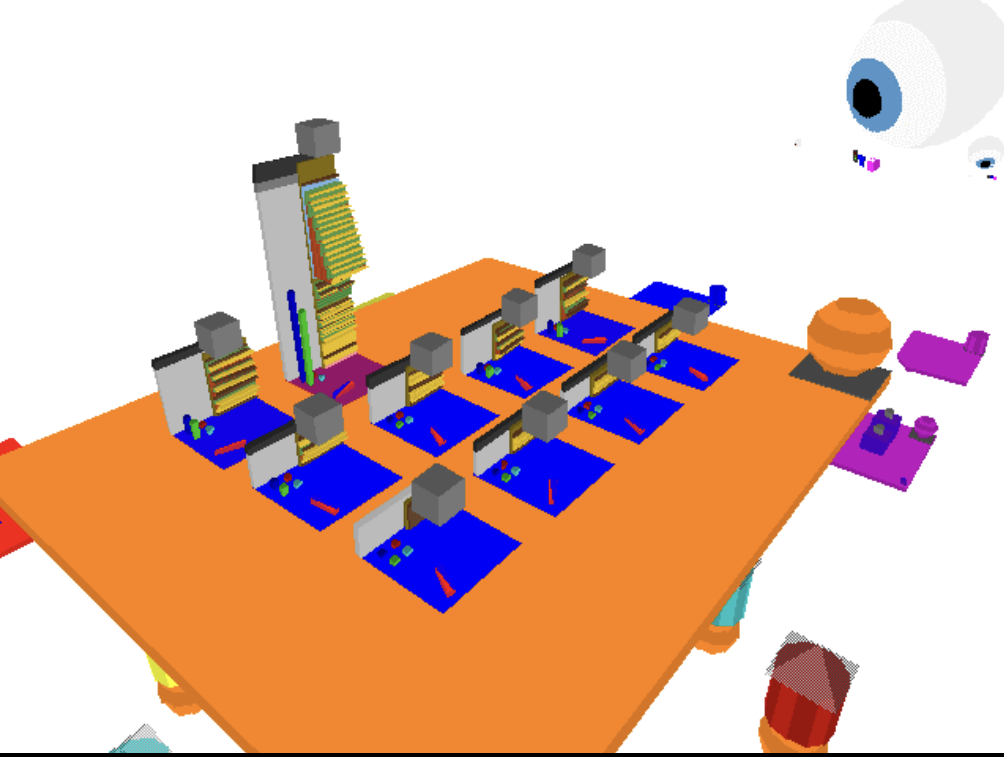
\includegraphics[width=0.5\textwidth]{images/visVRExample.png}
    \caption{Beispiel für eine 3D-Visualisierung von Young und Munro \cite[6]{visSoftwareVR}}
    \label{fig:3DVis}
\end{figure}

Trotzdem können wir auch für unser Ziel der Software-Qualitätsmetrik-Visualisierung Kriterien ableiten, die für eine gute Visualisierung wichtig sind \cite{visSoftwareVR}:
\begin{itemize}
    \item \textbf{Darstellung}: Der wichtigste Aspekt ist die Darstellung der Software. Die Visualisierung sollte die Struktur und den Aufbau der Software verdeutlichen. Die Frage ist also, wie wird die Software dargestellt? 
    \begin{itemize}
        \item Informationsgehalt: Die Visualisierung sollte so viele Informationen wie möglich enthalten.
        \item Niedrige visuelle Komplexität: Als Gegenspieler zum Informationsgehalt steht die visuelle Komplexität. Die Visualisierung sollte so einfach wie möglich gehalten werden, um den Betrachter nicht zu überfordern.
        \item Skalierbarkeit: Die Visualisierung sollte auch bei großen Software-Systemen noch gut lesbar sein. Dies ist besonders wichtig, da wir hier über große Software-Systeme sprechen. Die Autoren von \textit{Visualising Software in virtual reality} \cite{visSoftwareVR} sagen zudem, dass mechanismen Nötig sind, um Komplexität und Informationsgehalt zu steuern und je nach Software-System anpassen zu können.
        \item Stabilität gegenüber Änderungen: Die Visualisierung sollte stabil gegenüber Änderungen in der Software sein. Das bedeutet, dass die Visualisierung sich nur so sehr wie nötig ändert, wenn sich die Software ändert, um eine Versions konsistente Vergleichbarkeit zu ermöglichen und bereits mit der Visualierung vertraute Nutzer nicht zu überfordern.
        \item Gute Visuelle Metaphern: Die Visualisierung sollte gute visuelle Metaphern verwenden, um bereits bekannte Konzepte zu verwenden, um die Software verständlicher zu machen.
    \end{itemize}
    \item \textbf{Abstraktion}: Das Ziel von Visualierung muss sein, unwichtige Details auszublenden und ein verständliches Modell der Software zu erstellen.
    \item \textbf{Navigation}: Da wir häufig über große Software-Systeme sprechen, kann es schnall passeiren dass Nutzer in der Visualisierung verloren gehen. Es muss also möglich sein, sich gut zurecht zu finden und intuitiv zu wissen, wo was ist, um so ein grfühl für die software zu erhalten.
    \item \textbf{Korrelation mit dem Code}: Die Visualisierung sollte eine gute Korrelation mit dem Code haben. Wenn man die Visualierung sieht, soll man diese auch mit dem Code in Verbindung bringen können. Es sollte also möglich sein, die Visualisierung mit dem Code zu verknüpfen und so ein besseres Verständnis für die Software zu bekommen.
    \item \textbf{Automatisierung}: Die Visualisierung sollte automatisiert werden können - ein Punkt der trivialier weise gegeben ist, da wir hier über algorithmen sprechen, die keine manuelle eingabe benötigen.
\end{itemize}

\subsubsection{CodeCity} \label{sec:CodeCity}
Der Cornerstone von 3D Software-Qualitätsvisualisierung ist das Konzept von CodeCity \cite{codeCity1}. Das Paper von Richard Wettel und Michele Lanza verbindet einige Aspekte, die zu diesem Zeitpunkt neu waren. Sie reden zwar nicht konkret von software-qualitäts-visualierung, nutzen aber trotzdem qualitätsmetriken auf Klassenebene, um die richtige Granulariät von Software visualierung zu finden. Herkommliche paper waren oft noch auf niedrigeren ebenen z.b. Marcus Adrian et al. auf Ausdrucks-Ebene \cite{3dsoftwareMarcus}. Zudem nutzen sie, wie von Young und Munro \cite{visSoftwareVR} gefordert, eine gute visuelle Metapher, um die Software darzustellen. Sie nutzen das Konzept einer Stadt, um die Software darzustellen. Dabei wird jede Klasse als Gebäude dargestellt, dabei hat jedes Artefakt (Klassen, Pakete und Ordner) verschiedene Attribute: Die Dimension, die Position, die Farbe, die Farbsättigung und die Transparenz. Ein Beispiel für eine solche Visualisierung ist in Abbildung \ref{fig:codeCity} dargestellt.

\begin{figure}
    \centering
    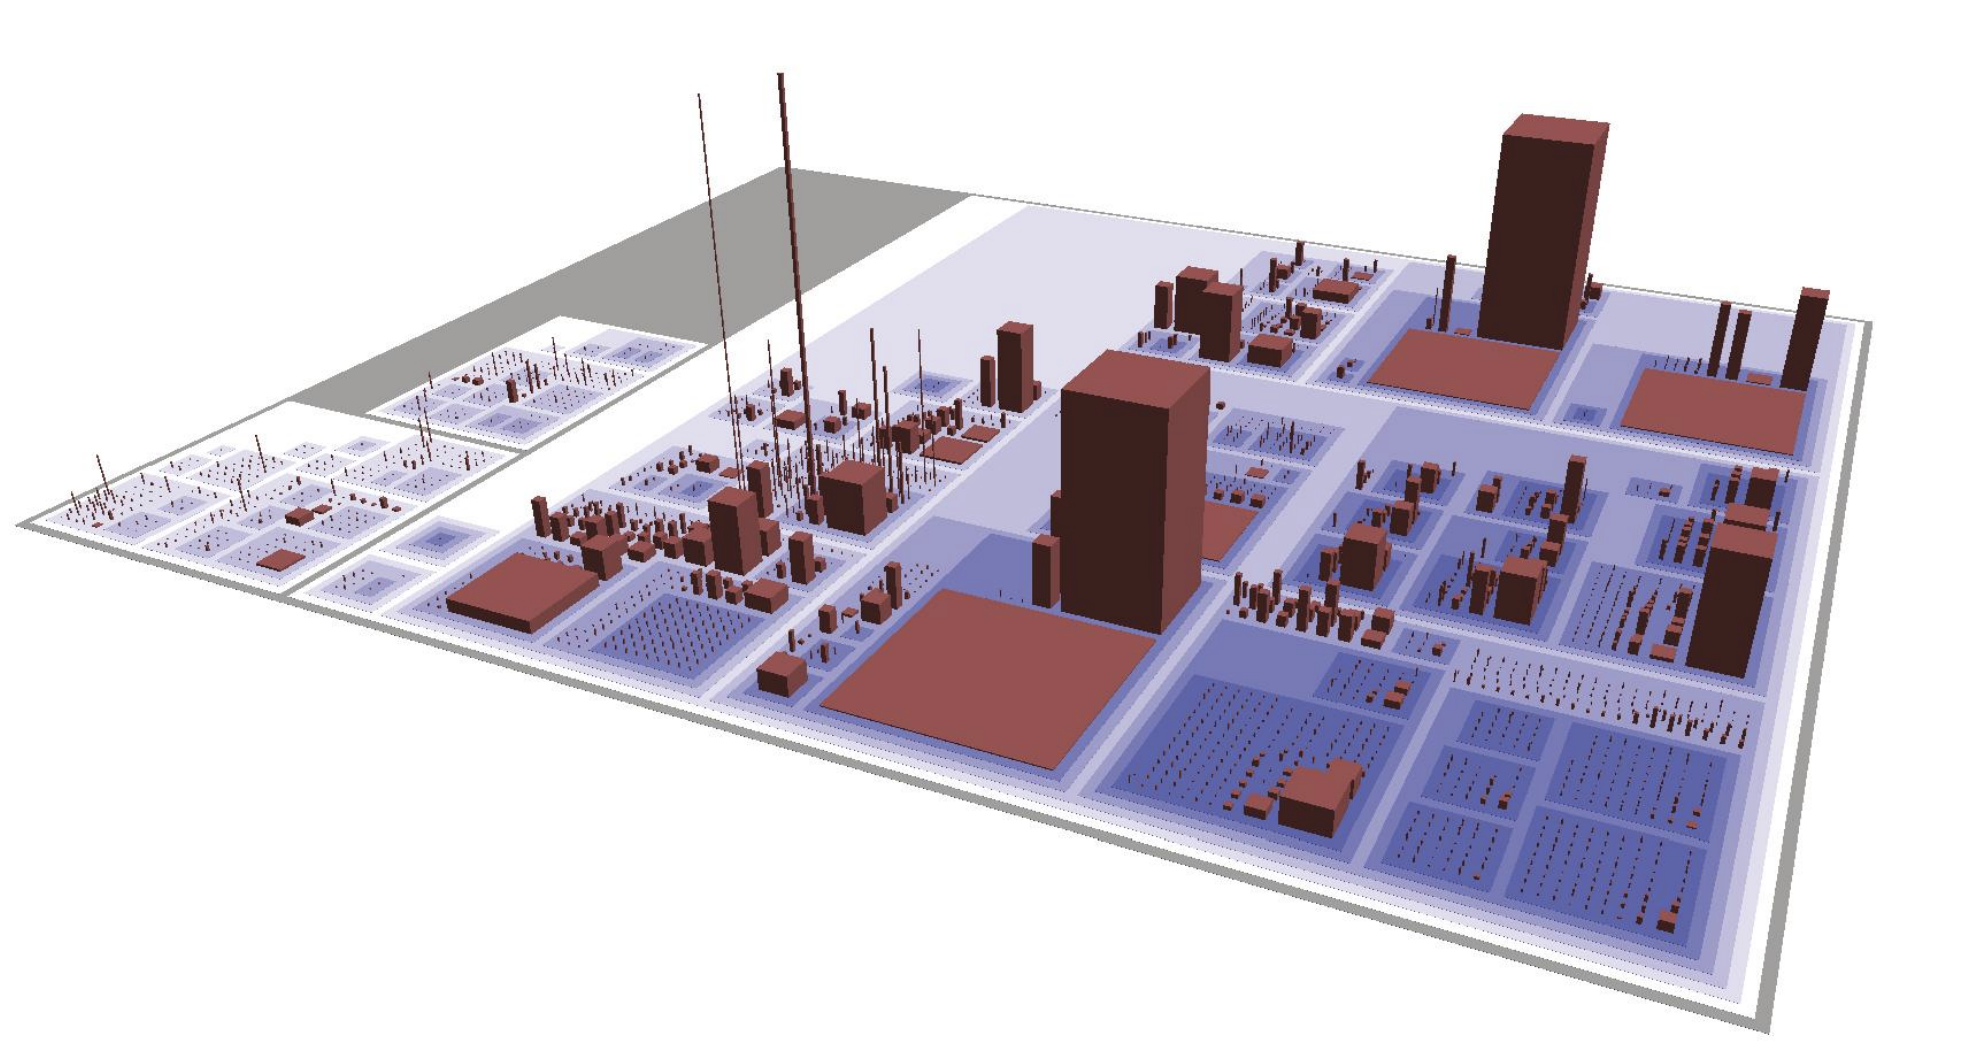
\includegraphics[width=0.5\textwidth]{images/codeCityExample.png}
    \caption{Beispiel für eine original CodeCity-Visualisierung \cite[2]{codeCity1}}
    \label{fig:codeCity}
\end{figure}

Das Layout der Stadt wird lässt sich dabei herunterbrechen auf ein 2D-Layout Problem. Um dieses problem zu lösen, implementieren sie eine abwandlung von Treemap-Algoithmen (Was treemaps sind wird in abschnit \ref{sec:Treemap} erklärt). Auffällig bei Ihrer implementierung ist, dass es viele ungenutzte leere flächen ohne gebäude gibt und gebäude anhand ihrer Größe sortiert plaziert werden (groß weiter unten links, klein weiter oben rechts). Leider ist der algotihmus nicht frei zugänglich, sodass in dieser Arbeit zum vergleich eine eigene Implementierung des Algorithmus verwendet wird, wodurch natürlich auch die Ergebnisse, von der original implementierung abweichen werden (außer wenn anders gekennzeichnet).

\subsection{Treemap-Layouts} \label{sec:Treemap}

Eine Treemap visualisiert einen Baum, indem jedem Knoten ein Rechteck mit der Fläche A zugewiesen wird, proportional zu seinem zugewiesenen Wert (z.B. Datenmenge oder Marktwert). Nicht-Blatt-Knoten werden dabei üblicherweise durch Rahmen (Container-Rectangles) gekennzeichnet, um die Gruppierung der Kinder zu zeigen. \cite{bruls2000squarified} Die Rechtecke aller Blätter füllen die Fläche des Wurzelrechtecks vollständig aus. Mathematisch entspricht die Eingabedatenstruktur einem gewichteten Baum, bei dem jede Blatteinheit eine numerische Größe hat. Die Fläche eines Eltern-Rechtecks entspricht der Summe der Flächen (Werte) seiner Kinder.

Die konkrete Idee hierarchische DAten in form von Treemaps darzustellen wurde erstmals 1991 von Shneiderman und Johnson \cite{johnson1991tree} vorgestellt. Sie stellten fest, dass die Darstellung von hierarchischen Daten in Form von Bäumen in der Regel nicht sehr anschaulich ist. Sie entwickelten eine Methode, um diese Daten in Form von Rechtecken darzustellen, die die Fläche der Knoten proportional zu ihrem Wert darstellen. Diese Methode wurde als \enquote{Treemap} bezeichnet. Als Ziele dieser Visualierung formulierten sie unter anderem diese Aspekte:
\begin{itemize}
    \item \textbf{Effiziente Nutzung des Platzes:} Generell soll es darum gehen möglichst viele Informationen auf einem kleinen Raum darzustellen.
    \item \textbf{Verständlichkeit:} Die Visualisierung soll so gestaltet sein, dass sie für den Betrachter leicht verständlich ist. Es soll möglich sein schnell und mit nur niedrigem kognitiven Aufwand die dargesllten Informationen zu erfassen.
    \item \textbf{Ästethik:} Die Visualisierung soll ansprechend gestaltet sein.
\end{itemize}

Zuvor bestehende Ansätze zur Visualisierung von hierarchischen Daten waren in der Regel nicht sehr anschaulich, besonders, wenn es um große Datenmengen ging. Listen, Baumdiagramme (siehe Abbildung \ref{fig:baumdiagramm}) oder andere Darstellungen (auch bekannt als Node oder Link-Diagramme) sind nicht in der lage alle diese Aspekte zu erfüllen. Bei Einem typischen Baumdiagram zum Beispiel werden teilweise mehr als die Hälfte der Fläche für Hintergrund genutzt \cite[3]{johnson1991tree} außerdem ist es schwer, außer der Struktur der Daten auch die Metriken darzustellen. Sie kritisieren auch die Darstellung von hierarchischen Daten in Form von Venn-Diagrammen (siehe Abbildung \ref{fig:venndiagram}): \enquote{The space required between regions would certainly preclude this Venn diagram representation from serious consideration for larger structures.}\cite[5]{johnson1991tree} Es ist zwar möglich durch die Größe der Kreise eine Metrik darzustellen, es sei aber nicht möglich eine große Anzahl an Knoten sinnvoll darzustellen. 

\begin{figure}[ht]
    \centering
    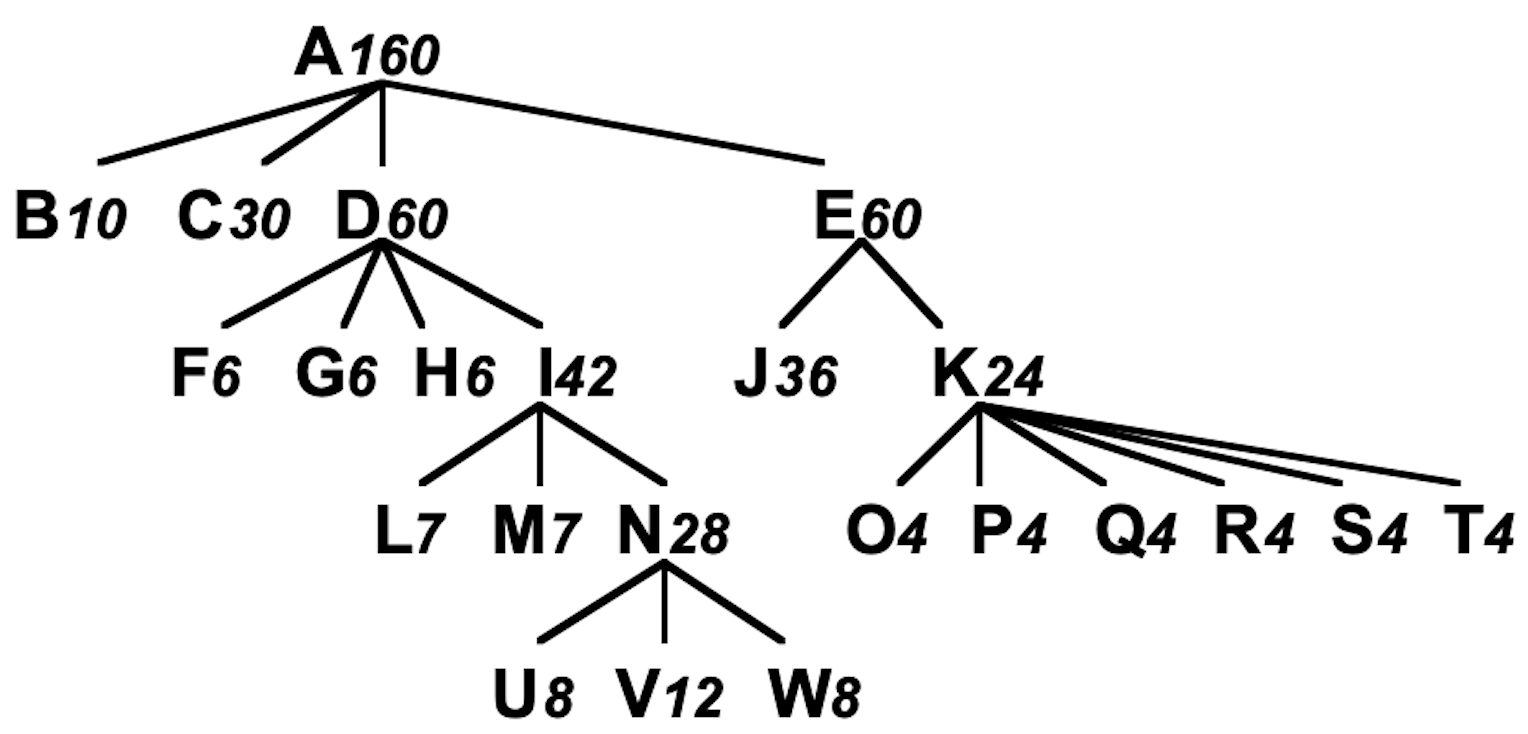
\includegraphics[width=0.5\textwidth]{images/treediagram.png}
    \caption{Beispiel für ein Baumdiagramm}
    \label{fig:baumdiagramm}
\end{figure}

\begin{figure}[ht]
    \centering
    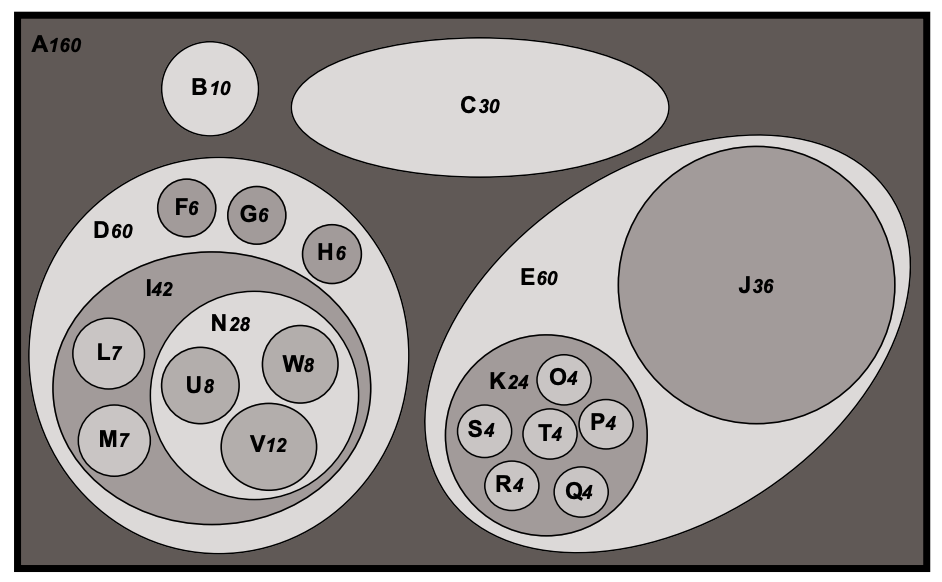
\includegraphics[width=0.5\textwidth]{images/verdiagram.png}
    \caption{Beispiel für ein Venn-Diagramm}
    \label{fig:venndiagram}
\end{figure}

\enquote{Using boxes instead of ovals and a bin-packing algorithm could partially solve this space
problem. But bin-packing is an NP-complete problem and does not preserve order.}\cite[5]{johnson1991tree} Sie stellen fest, dass es theoretisch eine dem Venn Diagramm ähnliche Lösung gibt, die allerdings NP-Hard ist. 

\begin{figure}[ht]
    \centering
    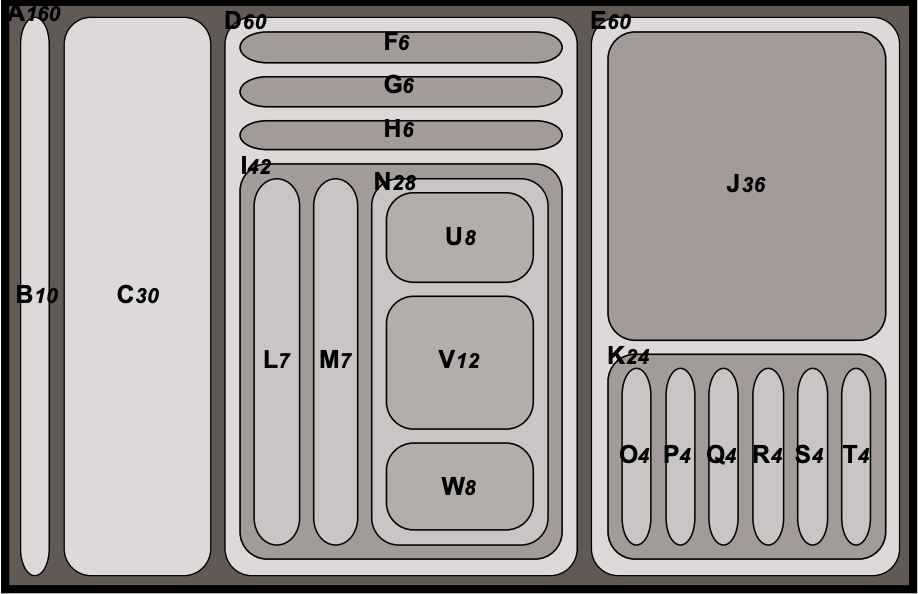
\includegraphics[width=0.5\textwidth]{images/rectVennDiagram.png}
    \caption{Beispiel für ein Boxed Venn-Diagramm}
    \label{fig:rectVennDiagramm}
\end{figure}

Shneiderman und Johnson schlagen zur Lösung dieser Schwierigkeiten ihren Treemap ansatz vor. Sie legen vier Eigenschaften fest, die bei der Erstellung der Treemaps gewährleistet werden:

\begin{itemize}
    \item Wenn ein Knoten 1 ein Vorfahre von Knoten 2 ist, dann ist der Bereich von Knoten 1 vollständig enthalten in dem Bereich von Knoten 2.
    \item Die Bereiche von zwei Knoten schneiden sich, wenn ein Knoten ein Vorfahre des anderen ist.
    \item Knoten belegen eine Fläche, die streng proportional zu ihrem Gewicht ist.
    \item Das Gewicht eines Knotens ist größer oder gleich der Summe der Gewichte seiner Kinder.
\end{itemize}

Sie stellen auch einen Algorithmus vor, der diese Eigenschaften erfüllen soll. Ein von diesem Algorithmus erzeugtes Layout ist in Abbildung \ref{fig:nestedTreemap} dargestellt. 

\begin{figure}[ht]
    \centering
    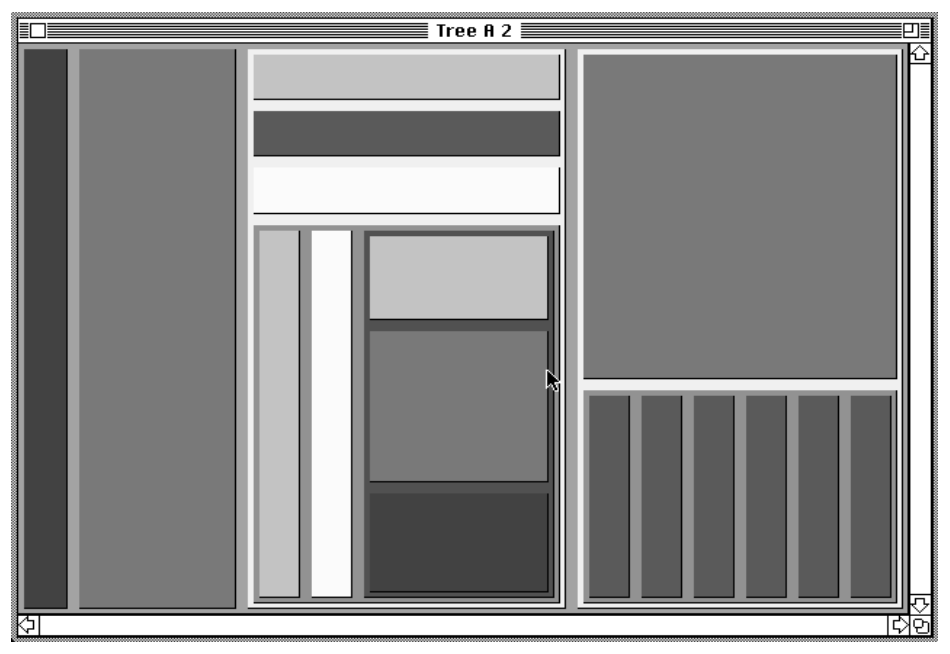
\includegraphics[width=0.5\textwidth]{images/nestedTreemapDiagramm.png}
    \caption{Beispiel für eine Treemap}
    \label{fig:nestedTreemap}
\end{figure}

Der Algorithmus unterteilt den Raum abwechselnd vertikal und horizontal, je nach größe der Knoten. Der Algorithmus arbeitet sich rekursiv von der Wurzel bis zu den Blättern herunter und hat eine Laufzeit von O(n), wobei n die Anzahl der Knoten ist. Im nächsten Abschnitt wird ein ähnlicher Algorithmus im Detail beschrieben, was zum besseren verständis dieser Art von Algorithmen helfen wird.

Obwohl es sich hier um ein renomiertes und viel Zitiertes Paper handelt, machen die Authoren einen entscheidenden Fehler, der in manchen Fällen sogar dazu führen kann, dass Rechtecke komplett verschwinden. Die Authoren betrachten dieses Problem in ihrem Paper leider nicht. 
Der Abstand zwischen den Knoten wird nämlich dadurch erzeugt, dass die Rechtecke diesen Abstand links, recht, oben und unten abgezogen bekommen. Dadurch ist die dargestellte Fläche der Rechtecke nicht mehr proportional zu den Werten, die sie darstellen sollen. Eigenschaft 3 wird also verletzt. Dies ist besonders problematisch, wenn die Rechtecke sehr klein bzw. sehr langgezogen sind. In diesem Fall kann es dazu kommen, dass die Rechtecke so klein werden, dass sie nicht mehr dargestellt werden können. Dies stellt in der Praxis ein riesiges Problem dar, speziell wenn das Problem dieser Arbeit also 3D im kopf bahalten wird. Es kann ja theoretisch vorkommen, dass als Flächenmetrik die lines of code verwendet wird und dort ein file, weil er wenige lines hat sehr klein wird und deswegen aufgrund der margins nicht angezeigt wird. Wenn jetzt aber die metrik für die Höhen berechnung die prozentualle test abdeckung der lines ist und der file nicht getestet ist, dann würde ein potentiell großes problem, was auch eigentlich direkt in auge springen sollte, nicht angezeigt werden. 

Ein weiteres Problem bei diesem Algorithmus ist auch generell, dass unter umständen die Rechtecke sehr langgezogen werden können, was unter Umständen auch Kriterium 3 der Ästethik verletzt. Es gibt viele Ideen dieses Problem anzugehen. Eine Möglichkeit, den Squarify Algorithmus zu verwenden, wird im nöchsten Abschnitt vorgestellt.

Zuletzt noch eine klarstellung im Bezug auf die erweiterung von 2D treemaps um eine Dimension. In der Literatur kommt es hier öfter zu unklarheit. Eigenlicht sind 3D treemaps so ähnlich wie 2D treemaps, nur dass sie anstatt ein rechteck zu unterteilen. Würfel bzw Quader unterteilen, wobei dann nicht die Fläche sondern das Volumen betrachtet wird. In dieser Arbeit geht es aber nicht darum, sondern um sogenannte 2.5D Treemaps, wobei das 2D Treemap layout nach oben extrudiert wird, um eine dritte Dimension zu erhalten. Wenn in dieser ARbeit also von 3D Darstellung die Rede ist, dann ist damit im Kontext von Treemaps eigentlich eine 2.5D Treemap gemeint.

\subsubsection{Squarify-Algorithmus} \label{sec:Squarify}

Der Squarify-Algorithmus ist ein Layout-Algorithmus für Treemaps, der darauf abzielt, die Fläche der Rechtecke so ausgewogen wie möglich zu gestalten. Beduetet, dass die Rechtecke möglichst quadratisch sind. Die ursprüngliche form des algorithmusses wurde im Jahr 2000 von Bruls et al. \cite{bruls2000squarified} vorgestellt. Sie stellten fest: \enquote{another problem of standard treemaps [is] the emergence of thin, elongated rectangles}\cite[1]{bruls2000squarified}. wenn rechtecke nicht mehr so langgezogen sind, Es ist einfacher auf Rechtecke zu zeigen, diese wahrzunehmen, sie zu vergleichen und ihre größe einzuschätzen. 

Der Algorithmus arbeitet rekursiv und teilt die Fläche in Rechtecke auf, wobei er versucht, die Seitenverhältnisse der Rechtecke so nah wie möglich an 1 zu halten. Sie stellen einen rekursiven Ansatz vor, bei dem, wie auch bei den meisten anderen Treemap-Algorithmen, die Rechtecke von oben nach unten (also vom Wurzelknoten bis zu den Blattknoten) aufgeteilt werden.

Im Folgenden wird der Algorithmus beschrieben, da er eine wichtige Grundlage für das Verständnis des Problems darstellt und außerdem eine gute Grundlage zum Verständnis der anderen Algorithmen bietet, da viele Algorithmen ähnliche Ideen verwenden.

Der Algorithmus wird anhand eines Beispiels aus dem originalen Squarify-Paper \cite[5]{bruls2000squarified} erläutert. Wir werden den Algorithmus jedoch anders erklären als im Paper, da wir uns näher an der Implementierung orientieren, wie sie in der bekannten d3-Bibliothek \cite{d3_treemap_code} umgesetzt ist.
Es sollen Rechtecke mit den Größen 6, 6, 4, 3, 2, 2, 1 in ein 6 mal 4 Rechteck einsortiert werden.

Der algorithmus arbeitet immer in Reihen, die er versucht zu füllen und dabei die Rechtecke möglichst quadratisch zu halten. Das erste Rechteck ist breiter als lang. (In dieser Arbeit werden wir, anders als in den herkömmlichen papern zu layout algorithmen, das Wort breit als x koordinate und das wort lang als y koordinate nutzen - das hat den hintergrund, dass das wort hoch im drei dimensionalen meist für die z komponent genutzt wird und es sonst zu verwirrungen kommen könnte)
Da das Rechteck in das wir einfügen breiter als lang ist, werden wir eine imaginäre horizontale Reihe so lange mit Rechtecken befüllen, bis ein Threshold erreicht ist. Das erste Rechteck mit größe 6 fügen wir also in Schritt 1 in diese Reihe ein. Das Seitenverhältnis dieses Rechtecks beträgt 8 zu 3 (das Rechteck ist 1.5 Einheiten breit und 4 Einheiten lang). Das zweite Rechteck mit größe 6 fügen wir in Schritt 2 in diese horizontale Reihe ein, dabei wird die Reihe entsprechend breiter. Das Seitenverhältnis des jetzt eingefügten Rechecks beträgt 3 zu 2 (das Rechteck ist 3 Einheiten breit und 2 Einheiten lang). Jetzt kommt das nächste Rechteck mit größe 4. Dieses Rechteck ist hat ein Seitenverhältnis von 4 zu 1 (das Rechteck ist 4 Einheiten breit und 1 Einheit lang). Das hinzufügen dieses Rechtecks führt nun aber dazu, dass das schlechteste Seitenverhältnis der Reihe von 3 zu 2 auf 4 zu 1 ansteigt. Deshalb wird diese Reihe als abgeschlossen angesehen und die nächste Reihe wird begonnen - Schritt 4. 

Dieser Schritt des suchens des schlechtesten Seitenverhältnisses lässt sich von der rechenkomplexität her gut optimieren, sodass der Ratio berechnet werden kann, ohne dass die Reihe wirklich mit Rechtecken gefüllt werden muss. 
Anstatt für jeder Rechteck max(w/l, l/w) zu berechnen, ziehen wir folgende vereinfachung heran.

\begin{align}
    \frac{w_i}{l_i} 
    &= \frac{w_i \cdot l_i \cdot w^2}{l_i \cdot l_i \cdot w^2} \\
    &= \frac{w_i \cdot l_i \cdot w^2}{l_i^2 \cdot \left(\sum_{j=0}^{n} w_j\right)^2} \\
    &= \frac{w_i \cdot l_i \cdot w^2}{\left(l_i \cdot \sum_{j=0}^{n} w_j\right)^2} \\
    &= \frac{w_i \cdot l_i \cdot w^2}{\left(\sum_{j=0}^{n} l_i \cdot w_j\right)^2} \\
    &= \frac{w_i \cdot l_i \cdot w^2}{\left(\sum_{j=0}^{n} l_j \cdot w_j\right)^2}
    \quad\text{da } \forall i, j \in \{0, \dots, n\}, l_i = l_j \\
    &= \frac{V_i \cdot w^2}{sV^2}
\end{align}
Analog dazu gilt das gleich auch für $ \frac{l_i}{w_i} = \frac{sV^2}{V_i \cdot w^2} $. Da wir nur an dem maximalen Wert beider Ausdrücke interessiert sind und die Länge ($l_i$) aller Rechtecke in der Reihe gleich ist, reicht es den Wert für das größte und das kleinste Rechteck zu berechnen und davon den maximalen Wert zu nehmen.

$w$ ist für den gesamten Zeitraum des füllens einer Reihe konstant und muss daher nur einmal berechnet werden. $sV$ wird mit jedem Rechteck aktualisiert. 

Das Ziel ist es das Verhältnis der Seitenlängen gleich zu halten. Im ursprünglichen Paper von Bruls et al. \cite{bruls2000squarified} wird darauf noch nicht so eingegangen, aber viele implementierungen z.b. die von d3.js \cite{d3_treemap_code} ermöglichen es, das Verhältnis nicht nur an den Wert 1 anzunähern, sondern auch an andere Werte, zum Beispiel den goldenen Schnitt \cite{goldenRatio}. 

\begin{figure}[h]
    \centering
    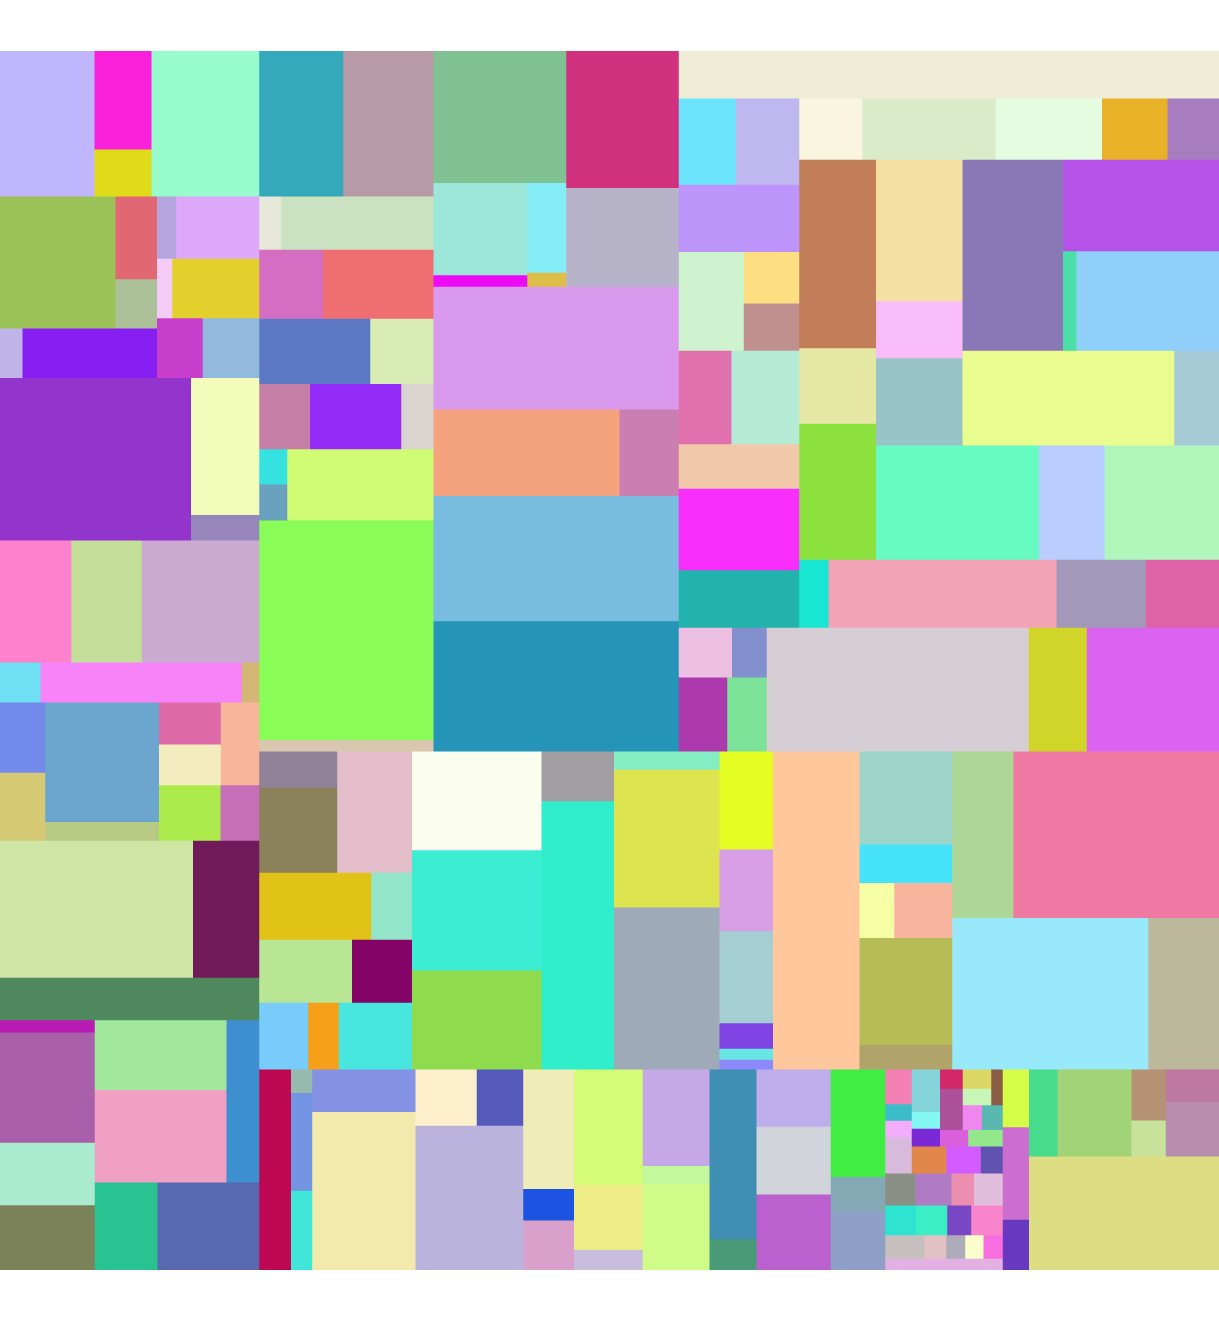
\includegraphics[width=0.5\textwidth]{images/oneSquarify.png}
    \caption{Beispiel für ein Squarify-Layout mit Annäherung an quadratische Rechtecke (Durchschnittliches Seitenverhältnis 1.42)}
    \label{fig:squarifyRatio1}
\end{figure}

\begin{figure}[h]
    \centering
    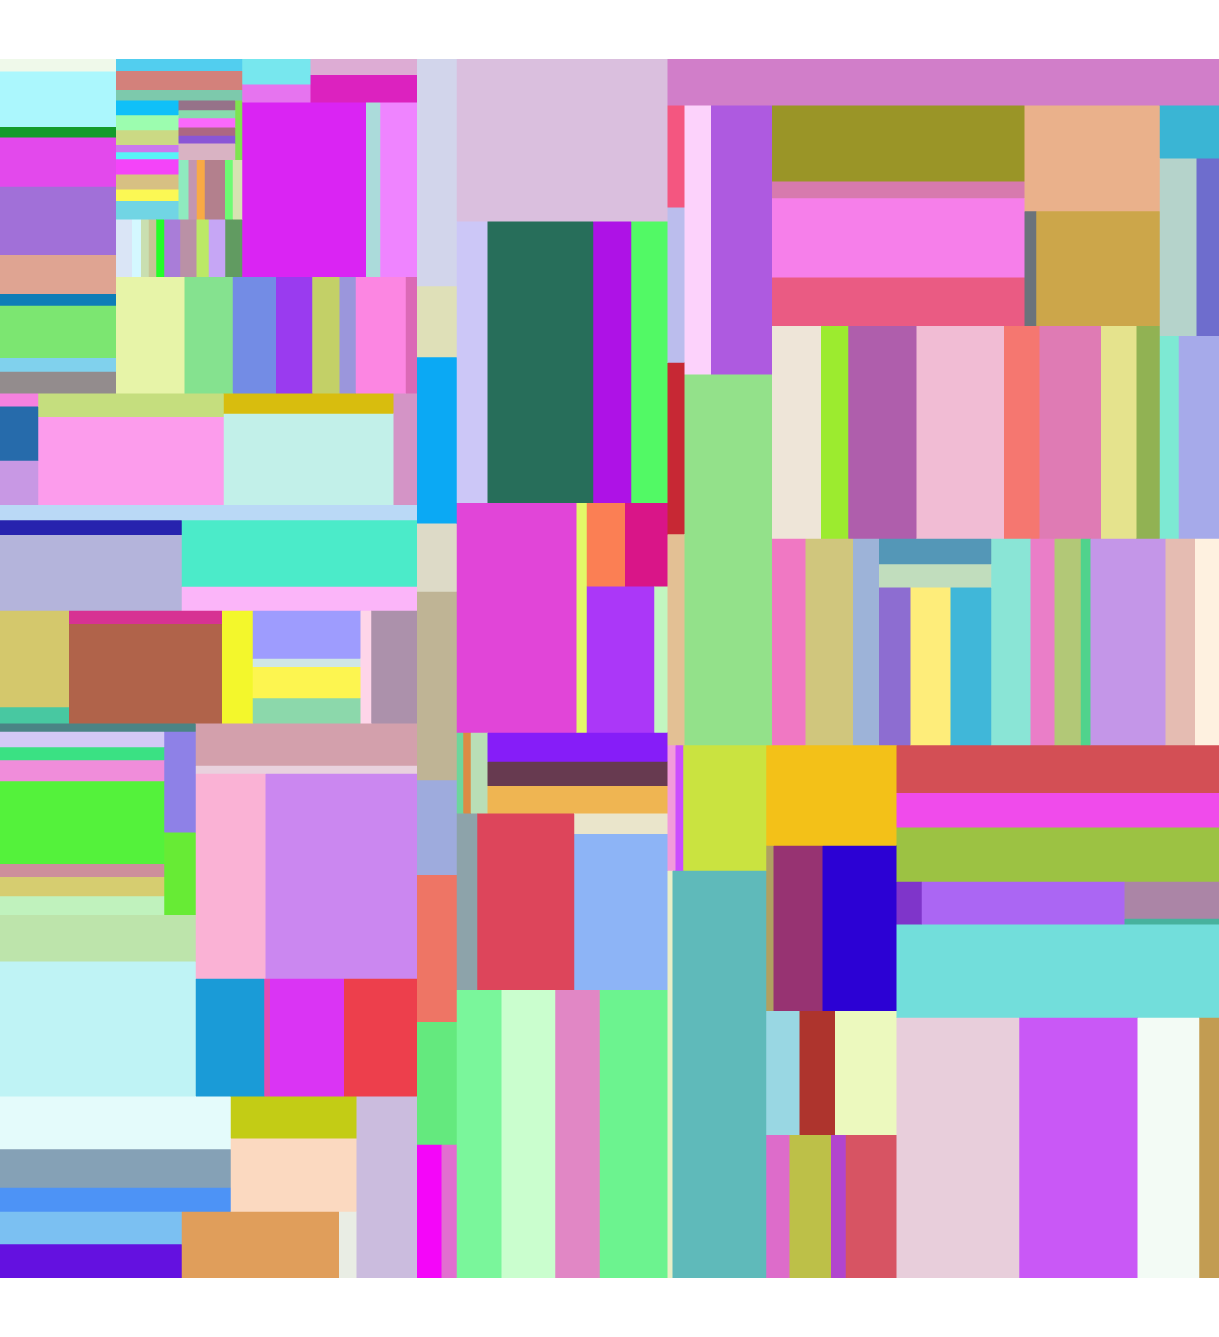
\includegraphics[width=0.5\textwidth]{images/fiveSquarify.png}
    \caption{Beispiel für ein Squarify-Layout mit Annäherung an den Wert 5 (Durchschnittliches Seitenverhältnis 2.79)}
    \label{fig:squarifyRatio5}
\end{figure}

%wie wirkt sich die reihenfolge auf das layout aus?
%was ist mit kd-bäumen